\chapter{Introduction}
\label{ch:intro}
With the increasing size of integrated
circuits, sequential circuit designers face complicated problems of
design errors in specification models and implementations. These
errors are usually modeled as ``bad" states, and the
circuits/functional components are modeled as finite state machines
(FSMs). Once state reachability is analyzed, the existence of errors
can be identified by checking whether ``bad" states are {\it
  reachable} from certain initial states. Temporal logic {\it model
  checking} (MC) formulations and solvers are often used for this
purpose. Once the designs and specification models are validated using
model checking, optimized implementations of sequential circuits are
synthesized. A subsequent problem then needs to be solved to prove
that the sequential circuit implementations are equivalent to the
original specification models, i.e. {\it Sequential Equivalence
  Checking   (SEC)}. When the specification is given as an arithmetic function
which canonically represents the circuit, then the problem 
becomes {\it functional verification} of sequential arithmetic circuits.

Reachability analysis forms the backbone of most sequential
verification techniques. As the state-space of FSMs increases,
reachability analysis forms a fundamental bottleneck in sequential
verification. Contemporary approaches employ various techniques to
overcome this state-explosion problem: 

\begin{enumerate}[{1)}]
\item Bounded model checking
\cite{bitlevel1} traverses the FSMs for a fixed number of steps $k$
($k$-BMC) to check whether a property violation can occur in $k$ or
fewer steps.  
\item Analyze over-approximations (or {\it abstractions})
of the state-space. Abstraction proves properties on the system by
first simplifying it, and when the abstraction does not satisfy the
same properties as the original one, a process of refinement is
needed. For example, counterexample guided
abstraction refinement (CEGAR) \cite{cegar-journal} uses proofs of
unsatisfiability (UNSAT cores) to refine the abstractions.
\item The recent breakthrough method of \cite{bradley2011sat} where the set of
over-approximations to forward reachable states are refined with
inductive constraints -- property directed reachability (PDR). 
\end{enumerate}

While the above techniques have made significant strides in sequential
verification, numerous practical instances remain unsolved. One issue
with all of the above techniques is that they mostly use bit-level
constraints to model the transition relations and sets of 
states. We have access to instances from our industrial
collaborators (Calypto Design Systems, now Mentor Graphics) where
the designs are expressed at the level of bit-vector words
(e.g. Matlab code, Verilog), and these word-level abstractions are
rarely exploited in verification. The problem is further exacerbated
when there are arithmetic operators on word-level operands embedded in
the control logic. While attempts have been made towards word-level
predicate abstraction \cite{jain2005word} \cite{mcmillan:cav06}
\cite{mcmillan2010lazy}, {\it using a purely word-level representation
  of the state-space, the properties and their abstractions have not
  been fully explored as another dimension in improving sequential
  verification.}  


For word-level SEC, we are given two designs, or their corresponding
Mealy/Moore FSMs ${\mathcal{M}}_1,{\mathcal{M}}_2$, along with their
initial starting states $S_0^1,S_0^2$. We wish to prove the absence of
a sequence of inputs (string) that distinguishes the initial
states \cite{coudert:iccad90}
\cite{coudert1990verification}. Fundamentally, this requires 
the construction of a product machine; and the main research problem
relates to that of performing {\it FSM traversal} \cite{touati1990implicit}
but  at the word-level. Analogously, in the case of MC, the problem
is setup w.r.t. a FSM $\mathcal{M}$, a set of initial states $S_0$ and
a set of property states $p$. Techniques are to be researched that
verify that there exist no sequence of transitions from an initial
state to a non-property state (``bad'' state). These problems have to
be solved in the context of word-level verification -- i.e. data
representation, abstraction using UNSAT cores and
algorithm execution has to be carried out at word-level.   




\section{Hardware Design and Verification Overview}
Following the Moore's law, the level of integration on modern VLSI becomes very high, 
such that a single digital VLSI design can implement a true system-level component.
The design process also evolves from manual design with little validation, to 
a formal 3-step procudure which needs collaboration of team with large number of 
engineers. The 3 major steps are: 1) Design, which is to specify and enter the design intent;
2) Implement, which is to refine the design through all phases with the assistance of Computer-Aided-Design (CAD)
tools; 3) Verify, which is to verify the correctness of design and implementation.

Nowadays the verify step is usually completed by a team with specialities on test, verification and validation of 
circuits. This step is also automated as an indispensable part of CAD tools, when circuit synthesis is performed. 
Figure \ref{fig:designflow} shows the typical synthesis flow, which covers all procudures starting from 
register-transfer-level (RTL) description (using hardware design languages, i.e. HDL) to  the 
physical design on silicon (depicted by the layout). The objective of verification in synthesis is 
to ensure the implementation is consistent with the original design intent. Verification is 
an important quality control measure before sending design layout to the VLSI foundaries.
Considering the high cost of fabrication, any faults and errors in the design will bring considerable 
waste of funds for the designers. On the other hand, all aspects of the society increasingly depend on 
the stability and accuracy of digital VLSI circuits, even small flaws or short-time failures can cause 
huge loss, especially in medical applications, military facilities and financial systems.
Therefore, it is of utmost importance to verify the correctness of VLSI designs.

One way to perform the verification is called {\it simulation}. It is defined as the collage of all circuit validation 
methods which apply stimulations on the inputs of circuit model and verify correctness of the outputs.
However, simulation is not a complete solution to circuit verification problems. In modern designs with 
large number of logic components and complicated architecures, it is impractical to simulate all possible 
test vectors. Usually only test vectors that correspond to typical failures are selected in simulation, which 
cannot cover unexpected failure patterns caused by special inputs. The notorious Intel FDIV bug \cite{nicely:FDIV}
is a good example when simulation fails. Failure occurs when only 5 entries in an $84\times 16$ look-up table
(LUT) are activated,  which is rarely used in most divisions. Because of the limitation of simulation,  
test engineers from Intel failed to detect the bug,  which brought $\$475$ million dollors recalling bill
for the company. Thus,  new methods that can guarantee the correctness of the design are necessary to be explored.

{
\begin{figure}[h]
\centerline{
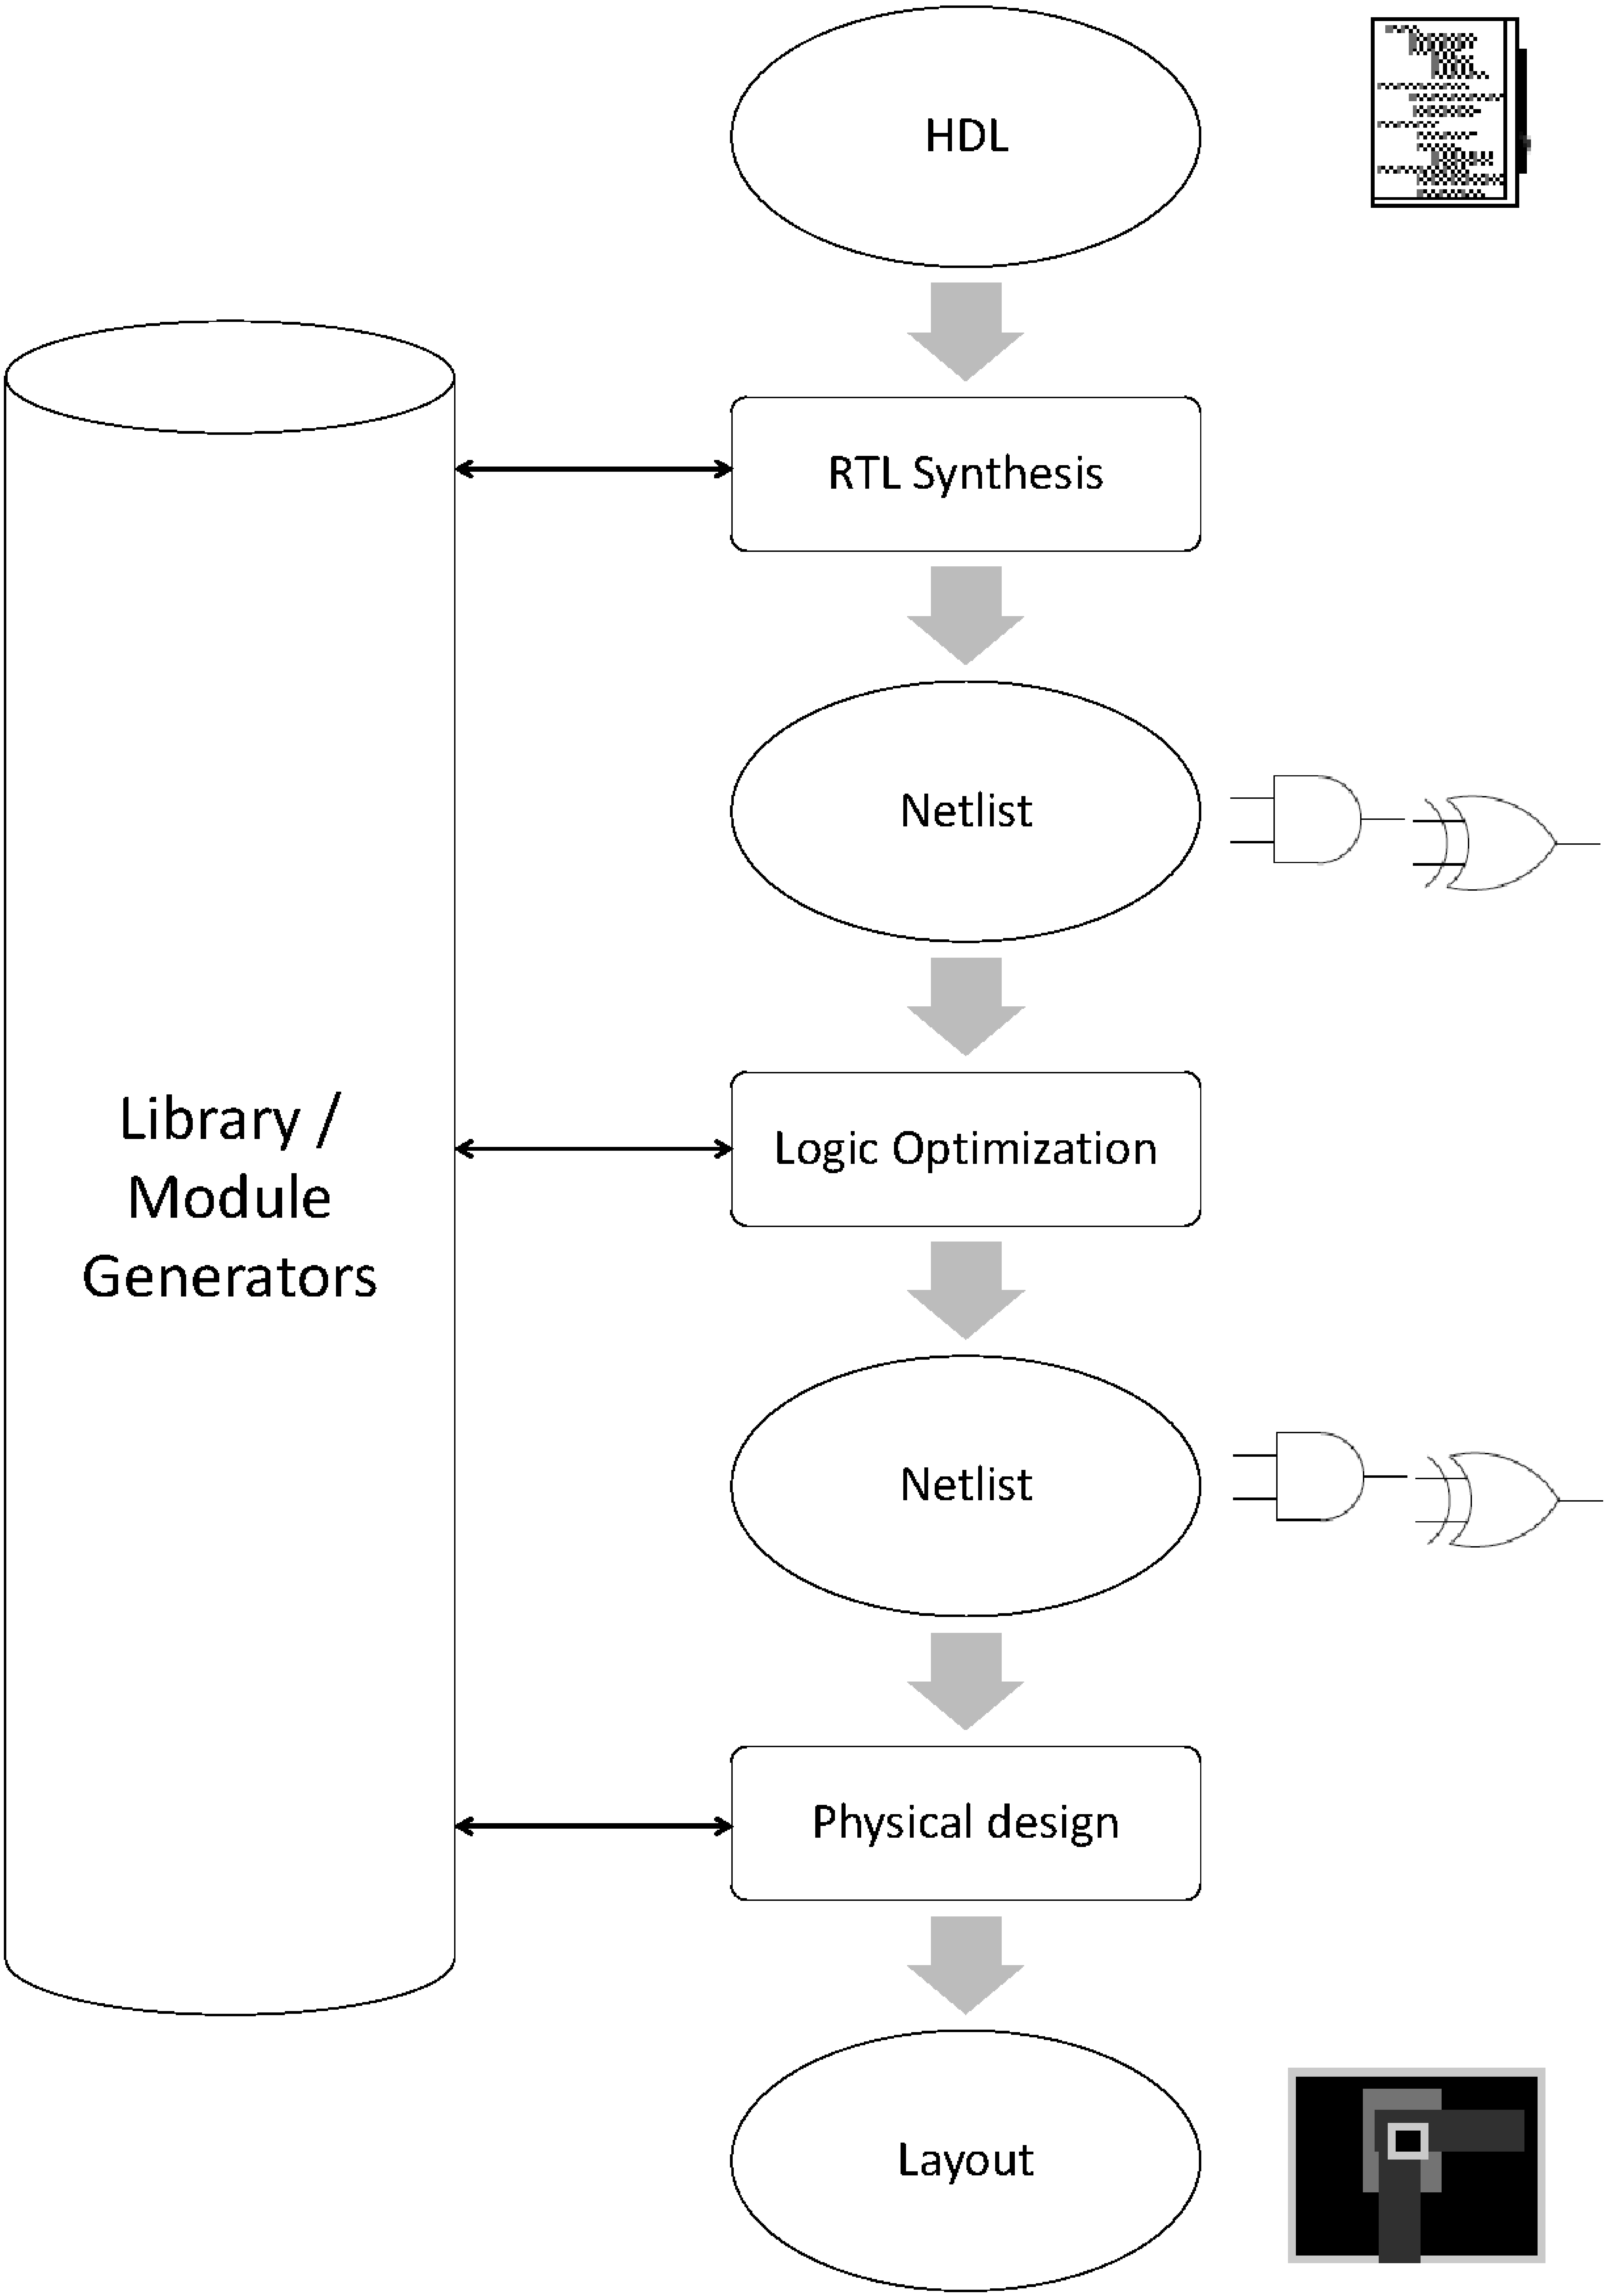
\includegraphics[width=0.7\textwidth]{newfig/designflow.eps}
}
\caption{Typical hardware design flow}
\label{fig:designflow}
\end{figure}
}


\section{Formal Verification}
% TODO this part require less modifications
Another method developed besides simulation is \emph{formal verification}, it utilizes 
mathematical theory to reason about the correctness of hardware designs.
Formal verification can provide $100\%$ fault coverage from 2 aspects. On the one hand,  it formalize properties
for the circuit model which are irrelevant to specific input signals,  and prove them mathematically.
On the other hand,  it adopts formal languages to strictly describe the design intents and detailed implementation, 
and deduces circuit function from the implementation. These descriptions are named as {\it specifications}.
Formal verification has two main forms: property checking and equivalence 
checking. 

{\it Property checking} (or property verification) verifies
that a design satisfies certain given properties. Property checking is done mainly 
in the form of theorem proving, model checking, or approaches which 
combine the two.
\begin{enumerate}
\item \emph{Theorem proving} \cite{theoremproving:91} requires the existence of
mathematical descriptors of the specification and implementation of the 
circuit. Theorem provers apply mathematical rules to these descriptors to
derive new properties of the specification. In this way, the tool can reduce
a proof goal to simpler sub-goals, which can be automatically verified.
However, generating the initial proof-goal requires extensive guidance from
the user, so there is an overall lack of automation in theorem 
proving.
\item \emph{Model checking} \cite{modelcheck:99} is an approach
to verifying finite-state systems where specification 
properties are modeled as a system of 
logic formulas. The design is then traversed to check if the 
properties hold. If the design is found to violate a
particular property, a counter-example is generated which exercises the
incorrect behavior in the design. Such counter-examples allow the designer
to trace the behavior and find where the error in the design lies.
Modern model checking techniques use the result to automatically refine
the system and perform further checking.
These tools are typically automated, and thus have found widespread 
use in CAD tool suites.
\end{enumerate}

{\it Equivalence Checking} verifies that two different representations of
a circuit design have equivalent functionality. An example of equivalence
checking as it applies to the hardware design flow is shown in
Fig. \ref{fig:equivflow}.

{
\begin{figure}[h]
\centerline{
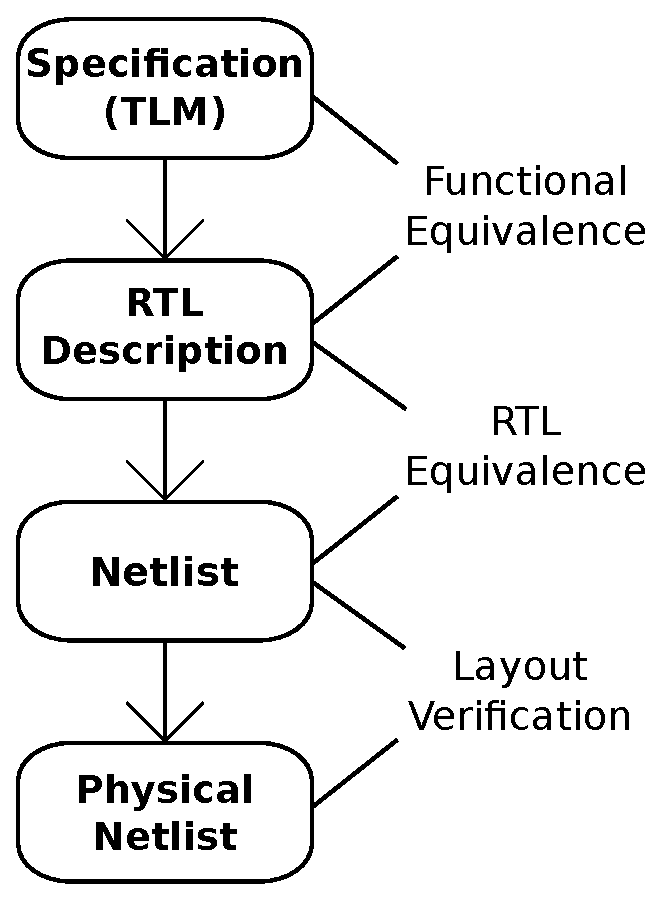
\includegraphics[width=0.5\textwidth]{./figures/designVerification}
}
\caption{Equivalence checking as applied to the hardware design flow.}
\label{fig:equivflow}
\end{figure}
}

There are two major
equivalence checking techniques: graph-based
and satisfiability-based.
\begin{enumerate}
\item \emph{Graph-based} techniques construct a canonical graph 
representation, such as a Binary Decision Diagram (\emph{BDD}) or one of
its many variants, of each circuit. A linear comparison is then conducted to 
determine whether the two graphs are isomorphic. Since the graph 
representation is canonical, the graphs of the two circuits will be 
equivalent if and only if the circuits perform the same function.
\item \emph{Satisfiability} techniques construct a miter of the two circuits,
typically in a graph such as an And-Inverter graph (\emph{AIG}). A
\emph{miter} is a combination of the two circuits with one bit-level output, which 
is only in a "1" state when the outputs of the circuits differ given 
the same given 
input, as shown in Fig. \ref{fig:miter}. 
A satisfiability (\emph{SAT}) tool \cite{csat} 
is then employed to simplify the graph and find a solution to the miter, 
i.e. find an input for which the 
miter output is "1". If a solution is found, this solution acts as a 
counter-example of when the circuit outputs differ; otherwise the circuits
are functionally equivalent.
\end{enumerate}


{
\begin{figure}[h]
\centerline{
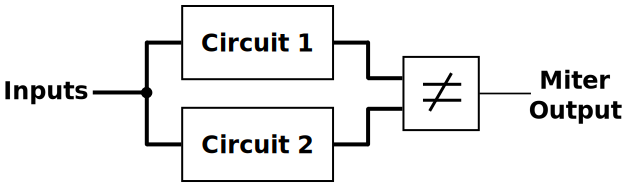
\includegraphics[width=0.8\textwidth]{./figures/betterMiter}
}
\caption{A miter of two circuits}
\label{fig:miter}
\end{figure}
}

%\subsection{Computer-Algebra Based Formal Verification}
Certain formal verification methods use \emph{computer-algebra} and \emph{algebraic
geometry} techniques based on mathematical theories.
Unlike SAT-based verification, modern algebraic geometry 
techniques do not explicitly solve the constraints to find a solution; 
rather, they reason about the presence or absence of solutions, or explore
the geometry of the solutions.
These methods \cite{Avrunin:CAV} \cite{condrat-tacas07} \cite{gbverify:2007} 
transform the circuit design into a polynomial system. Typically, this system
of polynomials is then used to compute a Gr\"obner basis \cite{gb_book}. 
Computation of Gr\"obner bases allows for 
the easy deduction of important properties of a polynomial system, 
such as the presence or absence of 
solutions. These properties are then leveraged to perform 
verification. Unfortunately, such a computation 
has been shown to be doubly 
exponential in the worst case, and thus these methods have not been 
practical for real-world applications. However, recent
breakthroughs in computer-algebra hardware verification have shown
that it is possible to overcome the complexity of this computation while
still utilizing the beneficial properties of a Gr\"obner bases
\cite{lv:phd}.

\section{Importance of Word-level Abstraction}
Most formal verification techniques can benefit from word-level abstractions 
of the circuits they verify.
There are several advantages in exploiting word-level information for
verification. A number of designs have  their
datapaths and/or system-level models described as word-level RTL
models.  Exploiting word-level instead of bit-level information is one
way of abstraction -- a key technique to reduce the state space of a
FSM. It has the effect of combining sets of states with similar 
properties. During reachability analysis, if we use bit-level
variables to  represent the states, the representations may become too
large to handle. However, when a ``bundle" of bit-level variables are
represented as {\it only one word-level variable}, the set of
reachable states can be represented by a  word-level constraint
expression; which may lower verification complexity.

% Abstraction is defined as state-space reduction, i.e{\text . }abstraction
% reduces state-space by mapping the set of states of a system to a smaller 
% set of states. Because the new representation contains fewer states, it
% is easier to comprehend and thus easier to use. 
% Word-level abstraction focuses specifically on abstracting a word-level
% representation of a circuit out of a bit-level representation. For example,
% a bit-level representation of an integer multiplier is represented by a
% collection of Boolean inputs and outputs, whereas a word-level
% abstraction hides the underlying logic and represents the circuit as two 
% integer inputs and one integer output, e.g. $Z=A\cdot B$. As the bit-size of the
% multiplier increases, the logical implementation of the multiplier grows (typically
% exponentially) while the word-level abstraction stays the same.

Word-level abstractions have a wide variety applications in formal 
verification. Theorem proving techniques can leverage abstraction as an 
automatic decision procedure or as a canonical reduction 
engine. For example, since RTL is composed of circuit blocks that represent 
the underlying circuit, RTL verification methods can exploit 
abstractions of these blocks.
This is seen in the following RTL verification methods:
\begin{itemize}  
\item Model checking \cite{kroening:model}, 
where an approximation abstraction of RTL blocks is generated and then 
refined.
\item Graph-based equivalence 
checking \cite{WLS} \cite{arditi:bmd}, where abstraction methods are used
to generate a canonical word-level graph representation of the circuit.
\item Satisfiability-based equivalence checking \cite{lpsat}, where 
abstractions are used identify symmetrics and similarities in order to 
minimize the amount of logic that is sent to the 
SAT tool. 
\end{itemize}

Other equivalence checking techniques that employ abstractions 
include satisfiability modulo theory ({\it SMT}) techniques \cite{boolector} \cite{bryant:tacas07}, 
which are similar to SAT except they operate on higher-level data
structures (integers, reals, bit vectors, etc.), as well as 
constraint solving techniques \cite {ms:research} \cite{tew:iccad08}.
In general, RTL equivalence checking approaches would ideally maintain a 
high-level of abstraction while still retaining sufficient lower-level 
functional details  (such as bit-vector size, precision, etc) 
\cite{gupta_survey}.

Word-level hardware abstractions also have applications in RTL and datapath 
synthesis \cite{demicheli:iccad_98} \cite{demicheli:dac_99}
\cite{demicheli:tcad_03}. 
Abstractions of circuits allow for design reuse, which allows for tool-automated 
synthesis of larger circuit blocks.
Since hardware design specifications tend to be word-level, synthesis tools 
can use these larger circuit blocks to generate and optimize the
datapaths and create the RTL of the system. Thus, in order for a circuit to 
be used by these automated synthesis tools, its word-level abstraction must
be known.

% Finally, abstractions can also be applied to detect malicious 
% modifications to a circuit, potentially inserted as a hardware trojan horse.
% Hardware trojans, a relatively new security concern in the hardware 
% industry, use certain techniques to add incorrect behavior to a 
% design. 
% This behavior is only activated under certain rare circumstances that only 
% the mal-intent designer has knowledge of.
% The behavior is purposely hidden and is very difficult to encounter during 
% simulation of the design. A manufactured chip with a subsystem 
% that contains a hardware trojan could compromise the entire system in which 
% it is used.
% In some hardware trojan cases, formal verification techniques may be applied 
% to catch a bug in a design and provide a counter-example which exercises it. 
% However, it can be difficult to tell whether the bug in the design was 
% introduced intentionally of not. On the other hand, word-level abstractions 
% of bit-level circuits {\it effectively reverse-engineer the true function 
% implemented by the circuit}, which could be used to determine the designer's 
% true intention.


\section{Objective, Motivation and Contribution of this Dissertation}
This research proposes a
set of new, promising approaches for {\it word-level representation,
reachability analysis and abstraction} with applications to SEC, sequential GF
arithmetic functional verification and 
$k$-BMC with abstraction refinement. Our techniques operate at the word-level and they are based
largely on the concepts from {\it algebraic geometry}. 

\subsection{Motivating Application}

The use of algebraic geometry
for sequential circuit verification and symbolic model checking has
been presented before. Avrunin presented the
concept of symbolic MC using algebraic geometry in
\cite{Avrunin:CAV}. Later, in \cite{vardi-iasted07}, Vardi presented
GB-algorithms for CTL, LTL and 
bounded MC over Boolean rings. However, these approaches are a
straight-forward transformation of the problem to {\it bit-level}
Boolean GB engines which are used in lieu of BDDs or SAT solvers. All
the concepts of word-level reachability, abstraction-refinement using
interpolation or UNSAT cores, etc., that we desire was not the focus of
\cite{Avrunin:CAV} \cite{vardi-iasted07}. 

{\bf The Algebraic Geometry Model and Rationale:} We will represent
the FSMs -- the transition relations -- by means of a set of
multi-variate polynomials with coefficients from the finite (Galois)
field $\Fkk$ of $2^k$ elements, i.e. polynomials in the ring
$\Fkk[x_1,\dots,x_d]$. Each state of a FSM is identified with a
Boolean assignment to a set of $k$-bit state register variables
$S=\{s_0,\dots,s_{k-1}\}$. Therefore, we can consider each ($k$-bit)
state as a word-level element $S$ of the finite field
$\Fkk$. Algorithms can directly operate on polynomials in word-level
variable $S$. 

Boolean functions with $k$-bit inputs and $k$-bit outputs 
$f: \B^k \rightarrow \B^k,\B = \{0, 1\}$ can be construed as functions
$f: \Fkk \rightarrow \Fkk$. It is well-known that over the finite
field ($\Fq$) of  $q$ elements, {\it every function} $f: \Fq
\rightarrow \Fq$ is a polynomial function \cite{ff:1997}. Moreover,
there exists a unique canonical polynomial $\Func$ that describes $f$.
This implies that one can derive a {\it  canonical, polynomial
  abstraction} of the function as $Z = \Func(A)$ where $Z, A$ are
word-level symbols representing $k$-bit operands. The concept also
generalizes to functions with different input/output bit-vector sizes,
i.e. functions of the type $f: \B^n \rightarrow \B^m$, modeled as
polynomials over $f:{\mathbb{F}}_{2^k} \rightarrow
{\mathbb{F}}_{2^k}$, where $k=LCM(n,m)$ \cite{ff:1997}.  
This implies that the FSM's transition relations can be
represented as polynomial functions (ideals) in $\Fkk$, and values of
state variables can be represented as solutions to these polynomials
(variety of the ideal). Subsequently, the ideal-variety correspondences
in algebraic geometry can be applied to implement symbolic reasoning
about state reachability. Moreover, as ${\mathbb{F}}_2 \subset \Fkk$,
our model provides a single, unified and bit-precise representation
for both bit-level (${\mathbb{F}}_2$) and word-level ($\Fkk$)
constraints.  

The decision and abstraction procedures in our setting will rely on
the theory and technology of {\it \Grobner bases (GB)}. GB-based
algebraic reasoning is very powerful; in fact it is known to be
strictly stronger than resolution \cite{CEI:stoc-96}. Therefore, in
light of the above discussion, using concepts from algebraic geometry
and \Grobner bases over $\Fkk$, we can introduce another dimension of
word-level abstraction to the techniques in sequential verification. 

\subsection{Dissertation Contributions}
% TODO revise this to contributions
In this dissertation, we focus on sequential circuit verification problems and 
propose solutions consisting of three main contributions: 
\begin{enumerate}[{1)}]
\item A method to perform reachability analysis at the word-level. 
	The given FSM is modeled as a system of polynomials over finite field,
	where the state space is mapped to its solution space.
	Our proposed algorithm utilize concepts in algebraic geometry including ideals and varieties.
	It also forms the foundation for word-level SEC and MC by enabling word-level abstraction of the
  state-space.
\item Using the theory of FSM traversal, we apply the algorithm to verify the 
function of sequential GF arithmetic circuits. Our proposed approach uses GB-engines efficiently 
and can verify sequential multipliers with 162-bit datapaths.
\item We explore the concept, and the computation, of unsatisfiable (UNSAT)
  cores of  a set of polynomials using Gr\"obner bases calculation. We apply the UNSAT core extraction 
  to abstraction-refinement
  techniques such as bounded model checking (BMC). 
\end{enumerate}

\section{Dissertation Organization}
The rest of the dissertation is organized as
follows: Chapter \ref{ch:prev} reviews previous work, and analyzes their drawbacks with respect to 
the word-level sequential verification problem.
Chapter \ref{ch:prelim_GF} covers preliminary
concepts and notation on finite fields, and the methodology about design of multipliers in finite fields.
Chapter \ref{ch:ideals} provides a theoretical background of algebraic geometry and Gr\"obner bases.
Chapter \ref{ch:reacha} describes the basic
concept of word-level FSM traversal and introduces our proposed word-level FSM traversal algorithm. 
Chapter \ref{ch:normal} explores the application of FSM traversal algorithm on 
functional verification of sequential GF arithmetic circuits. Chapter \ref{ch:UNSAT} describes
algorithmic techniques to derive UNSAT cores of polynomial
ideals. It also demonstrates with the help of an example how abstraction via
UNSAT cores in algebraic geometry can simplify BMC. 
Chapter \ref{ch:conclude} concludes the dissertation and outlines potential future research for
continuation of this work.